\documentclass{article}
\usepackage{graphicx} % Required for inserting images
\usepackage[margin=1in]{geometry}
\usepackage{amsmath}
\usepackage{amsthm}
\usepackage{amssymb}
\usepackage{amsfonts}
\usepackage{verbatim}
\usepackage{tikz}
\usepackage{xcolor}

\title{Final Project: Report}
\author{Dante Buhl}


\DeclareMathOperator{\cond}{cond}
\DeclareMathOperator{\vecspan}{span}
\DeclareMathOperator{\sign}{sign}
\DeclareMathOperator{\diag}{diag}
\DeclareMathOperator{\upper}{upper}
\DeclareMathOperator{\lowtri}{lower}

\begin{document}

\newcommand{\bs}[1]{\boldsymbol{#1}}
\newcommand{\bmp}[1]{\begin{minipage}{#1\textwidth}}
\newcommand{\emp}{\end{minipage}}
\newcommand{\R}{\mathbb{R}}
\newcommand{\C}{\mathbb{C}}
\newcommand{\N}{\mathcal{N}}
\newcommand{\I}{\mathrm{I}}
\newcommand{\K}{\bs{\mathrm{K}}}
\newcommand{\m}{\bs{\mu}_*}
\newcommand{\s}{\bs{\Sigma}_*}
\newcommand{\dt}{\Delta t}
\newcommand{\tr}[1]{\text{Tr}(#1)}
\newcommand{\Tr}[1]{\text{Tr}(#1)}

\maketitle



\section{Part A: Reduced Rank Image Reconstruction}
\begin{enumerate}
    
    \item

    The first ten largest singular values are $\{\sigma_{1} = 281897.27, \sigma_{2} = 46571.71, \sigma_{3} = 31487.79, \sigma_{4} = 26436.71, \sigma_{5} = 19631.55, \sigma_{6} = 15569.22, \sigma_{7} = 14390.26, \sigma_{8} = 11254.04, \sigma_{9} = 9660.39, \sigma_{10} = 9411.763 \}$. Furthermore the ``rest singular values'' are as follows $\{ \sigma_{10} = 9411.73, \sigma_{20} = 4167.18, \sigma_{40} = 2035.98, \sigma_{80} = 1193.12, \sigma_{160} = 758.44, \sigma_{320} = 456.38, \sigma_{640} = 189.13, \sigma_{1279} = 4.76\}$. 

    \item Here are the following eight images generated by the reduced rank approximation for the image. 

\begin{center}
    
    \begin{tabular}{| c | c |}
    \hline
    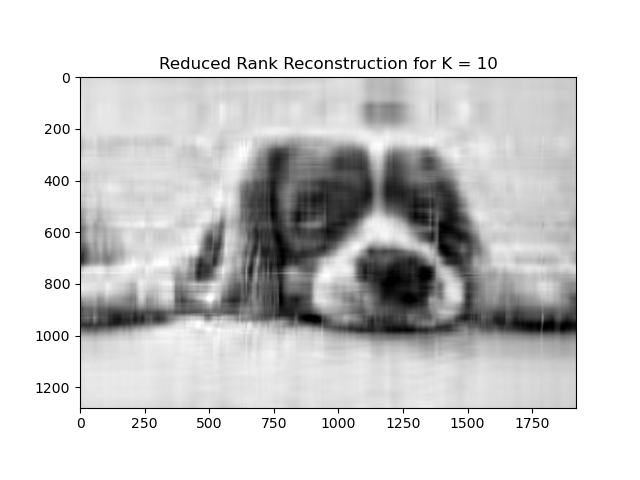
\includegraphics[width=.40\textwidth]{Image_appn_100010.png} & 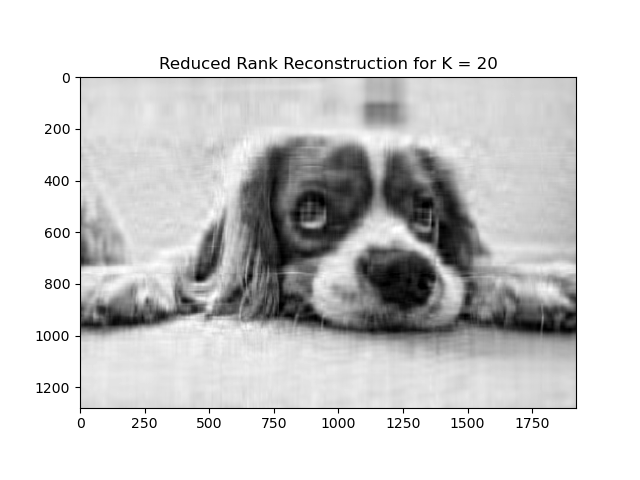
\includegraphics[width=.40\textwidth]{Image_appn_100020.png} \\
    \hline
    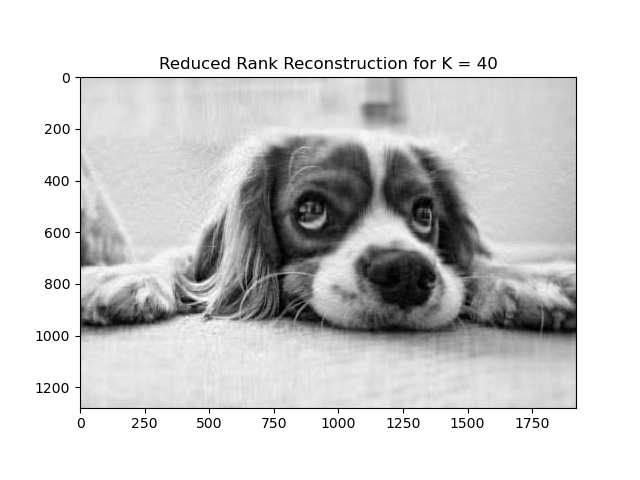
\includegraphics[width=.40\textwidth]{Image_appn_100040.png} & 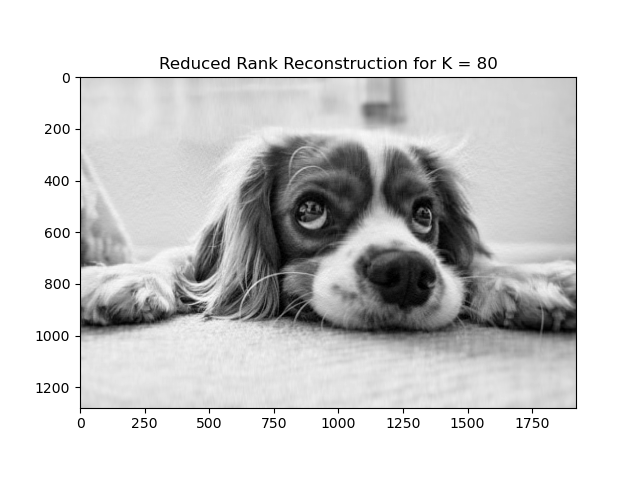
\includegraphics[width=.40\textwidth]{Image_appn_100080.png} \\
    \hline
    \end{tabular}

    \begin{tabular}{| c | c |}
    \hline
    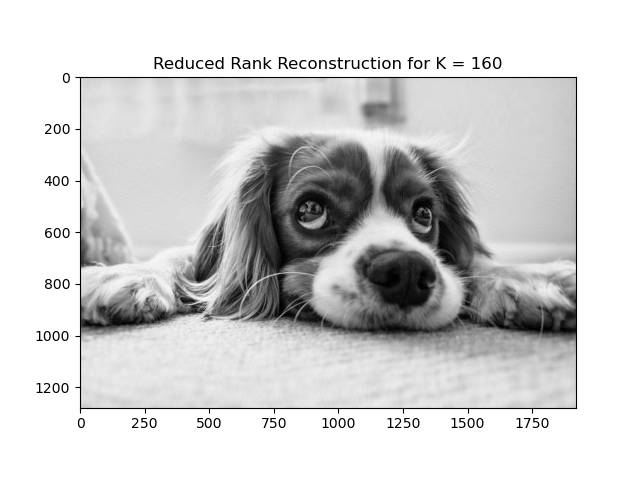
\includegraphics[width=.40\textwidth]{Image_appn_100160.png} & 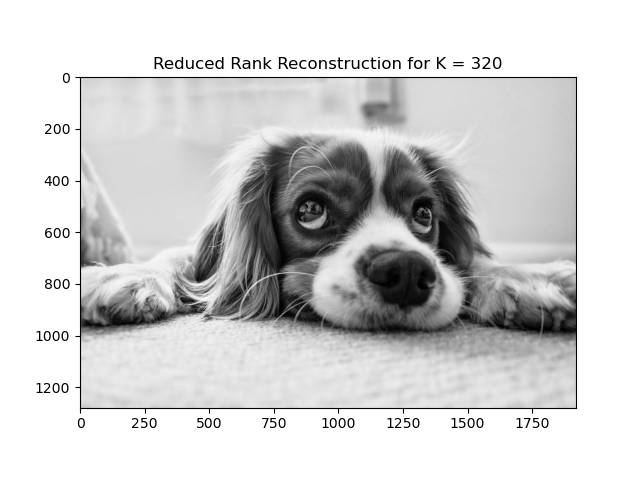
\includegraphics[width=.40\textwidth]{Image_appn_100320.png} \\
    \hline
    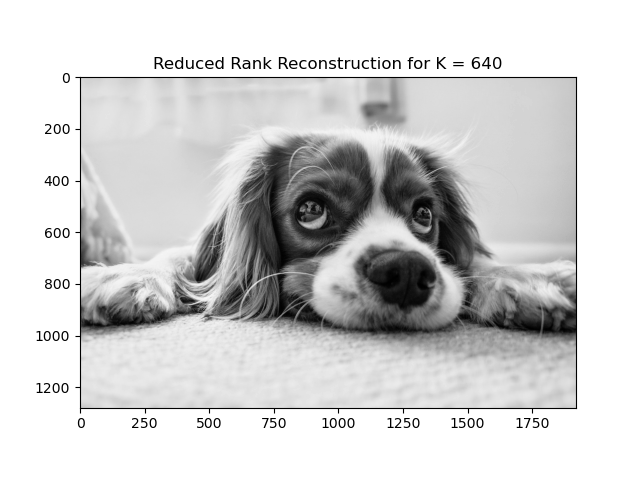
\includegraphics[width=.40\textwidth]{Image_appn_100640.png} & 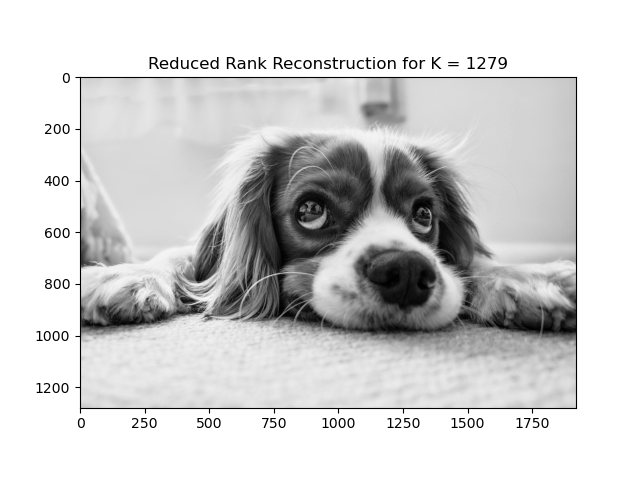
\includegraphics[width=.40\textwidth]{Image_appn_101279.png} \\
    \hline
    \end{tabular}

    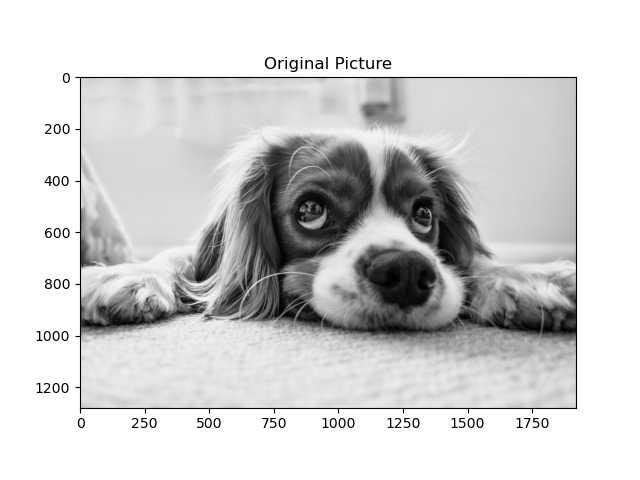
\includegraphics[width=.60\textwidth]{original.png}
\end{center}

    \item 

    It is easily noticable that as we reduce the rank of our appoximations more and more, that the quality of the image decreases. Some of the differences between rank approximations aren't as noticable as others. Between ranks of the reconstruction 40 and 80 there is a very noticable sacrifice in image quality. There seem to be smudges in the picture and a sort of typical graininess which is present in low resolution images. This is what is noticable here. Looking at the error reports of these approximations we find that we only find a normalized error below $10^{-3}$ for our rank 10 approximation. All other normalized errors are of order $10^{-3}$ or lower. The lowest being the rank 1279 error at $10^{-16}$ exactly the order of machine double precision. 

\end{enumerate}

\section{Iterative Methods}
\subsection{Gauss-Jacobi/Gauss-Seidel}

    \begin{enumerate}

        \item Both the Gauss-Jacobi and Gauss-Seidel methods involve an iterative method in which we recompute a vector x and after (hopefully) a finite number of iterations we will reach the desired level of error. They differ in the compution of the next x vector from the proceeding one. In Gauss-Jacobi, it is simply one line of matrix multiplcation and subtraction, i.e.
    \[
        x^{(n)} = D^{-1}(b - Rx^{(n-1)}), \quad D = \diag(A), \quad R = A - D
    \]
    This is much easier to compute since $x^{(n)}$ only depends on the givens $A, D, R, b$ and the previous iteration. A slightly more complex algorithm, Gauss-Seidel, is derived from this where we break $R$ into an upper and lower matrix, i.e.
    \[
        A = D + R + L, \quad D = \diag(A), \quad R = \upper\Delta(A - D), \quad L = \lowtri\Delta(A - D)    
    \]
    Here the iterative method is 
    \[
        x^{(n)} = 0 \to x_i^{(n)} = \frac{1}{a_{ii}}(b_i - L_{i, 1:i-1}x_{1:i-1}^{(n)} - R_{i, i+1:m}x_{i+1:m}^{(n-1)})
    \]
    Here we have that going down the elements of $x^{(n)}$ each element depends on the term before it. This means that rather than one line of matrix opertions, we have to express the iterative process for $x^{(n)}$ as a loop over the $m$ elements of the vector. For each method, the convergence criterion is slightly different. For the Gauss-Jacobi method we must have that $T = D^{-1}R$ has eigenvalues such that, $\rho(T) < 1$. This will guarantee that as we take the number of iterations to infinity, 
    \[
        x^(n) = Tx^{(n-1)} + c = T^2x^{(n-2)} + Tc^{(n-2)} + c^{(n-1)}
    \]
    \[
        x^{(n)} = T^{n}x^{(0)} + T^{n-1}c^{(0)} + \cdots + Tc^{(n-2)} + c^{(n-1)}
    \]
    \[
        \lim_{n\to\infty} x^{(n)} = const.
    \]
    The convergence criterion for Gauss-Seidel is similar, Gauss-Seidel will converge if Gauss-Jacobi converges and will converge faster, however there are cases where Gauss Seidel Converges but Gauss Jacobi does not. In the case of Gauss-Seidel a similar argument can be made but for $T = (D + L)^{-1}R$. We have, 
    \[
        x^{(n)} = Tx^{(n)} + c
    \]
    Notice that by Gergorin's theorem we will have that the eigenvalues of $D + L$ can be larger than the eigenvalues of $D$ and similarly, the eigenvalues of $R$ become constrained. Therefore we will have that the eigenvalues of $T$ will be lower than in the case for Gauss-Jacobi and therefore will converge faster. 

    \item

    Here are the plots obtained for all values of D. 

    \begin{center}
    
    \begin{tabular}{| c | c |}
    \hline
    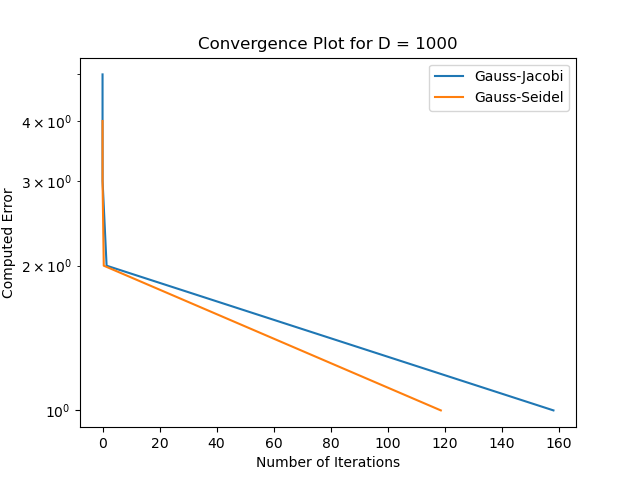
\includegraphics[width=.40\textwidth]{D1000plot.png} & 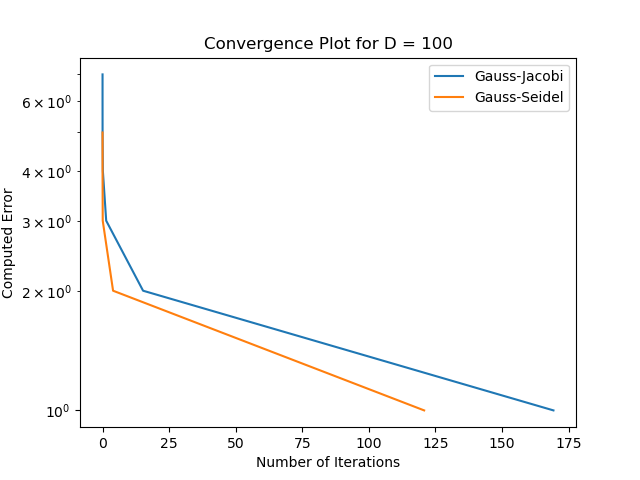
\includegraphics[width=.40\textwidth]{D100plot.png} \\
    \hline
    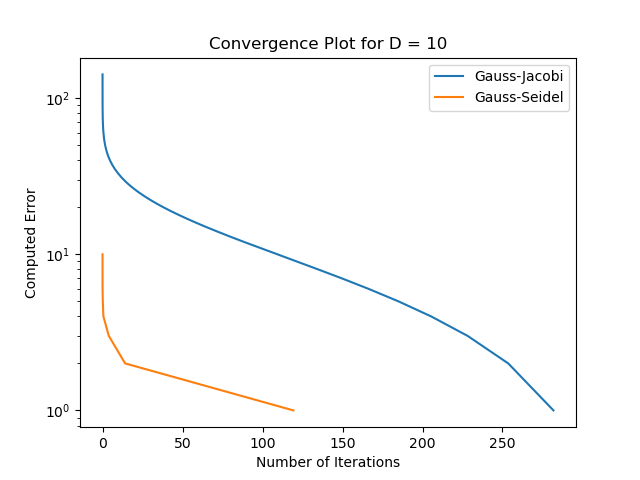
\includegraphics[width=.40\textwidth]{D10plot.png} & 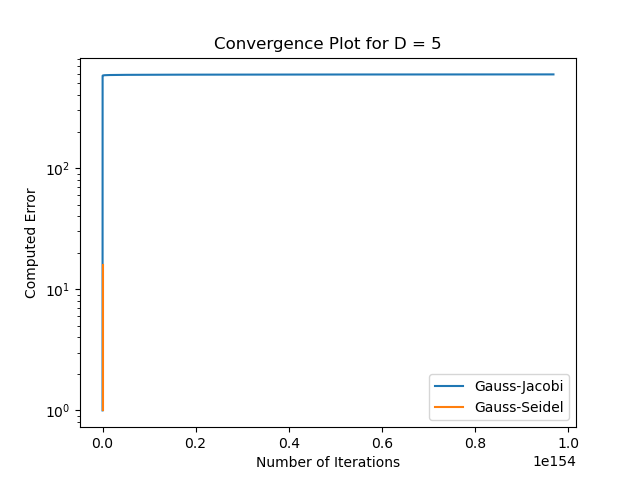
\includegraphics[width=.40\textwidth]{D5plot.png} \\
    \hline
    \end{tabular}
    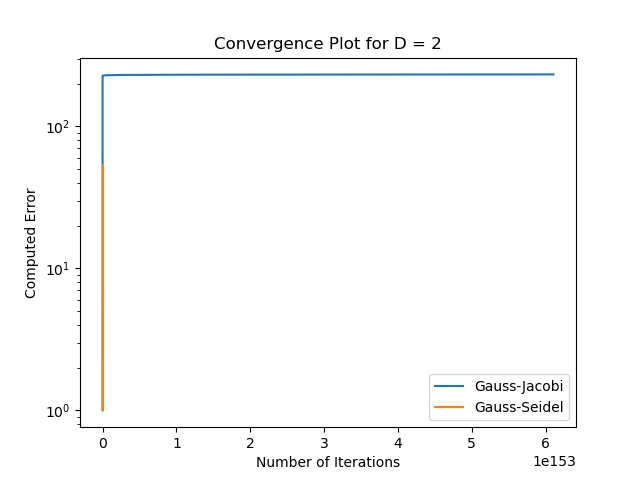
\includegraphics[width=.4\textwidth]{D2plot.png}
    
    \end{center}


    \item 
        
    Some of the cases didn't converge, specifically $D = 2$ and $D = 5$ for the Gauss-Jacobi method. For both of these cases the number of iterations reached into the order of $10^2$ and the final result is NaN, usually indicating an underflow. For the cases where both methods converge, we see that Gauss-Seidel converges more quickly. This matches the theoretical predictions that we went over in lecture yielding better convergence and stability for Gauss-Seidel with the trade off of not being able to parallelize. To investigate why this didn't converge, we look at the spectral radius of these matrices. Notice that for $D = 2$ we have that $D^{-1}R = \left[\begin{array}{c c} 0 & \bs{\frac{1}{2}} \\ \bs{\frac{1}{2}} & 0 \end{array}\right]$. For the case of $D=5$, we have, $D^{-1}R = \left[\begin{array}{c c} 0 & \bs{\frac{1}{5}} \\ \bs{\frac{1}{5}} & 0 \end{array}\right]$. In both cases we have from Gershgorin's Theorem, for the eigenvalues of $D^{-1}R$,
    \[
        |\lambda_{ii}| \le  4.5,\quad |\lambda_{ii}| \le 1.8
    \]
    Notice that for both cases of $T$ we have that the eigenvalues no not necessarily have to be below 1 and so the algorithm is not guaranteed to converge. 

    \item 
    For the case of $A_{ii} = i$ we have that the Gauss-Jacobi method does not converge, but Gauss-Seidel does. 

    \end{enumerate}

\subsection{Conjugate Gradient}

    \begin{enumerate}

        \item The Conjugate Gradient Method is a method similar to gradient descent where each iteration, there is a direction chosen and a step length along that direction such that each iteration the ``function'' will approach a local minimum. This ``function'' is chosen such that is contains the information of the system of equations that we are trying to solve. The reason we can pick such a method is because of the properties of martrices which this method applies to, specifically symmetric positive definite matrices. Finally, the reason why we are guaranteed to converge within $m$ iterations is because on each iteration we pick a distance along a vector which brings us as close as possible to the minimum. At the next iteration we choses a vector orthogonal to all previous vectors and get as close to the minimum once again. Since these vectors are orthogonal, we are guaranteed to never move in a direction parallel to a previous vector. Furthermore, we know orthogonal vectors (a cconjugate set") can be taken from $A$ which span $\R^{m}$ since its eigenvectors form an a basis for $\R^m$. Since there are at most $m$ vectors in the basis, we have that after $m$ iterations we will be out of vectors to chose from, and thus (if we did out work properly) we will have reached the minimum of the function, and thus the most accurate approximate solution to $Ax = b$. 
    
        \item 

        \begin{proof}
            To prove the two algorithms are identical we must look closely aat the differences between the two methods. First we notice that the "smart" method relies on two quantities called $E$ and $E_{\text{new}}$. These quantities serve the purpose of holding onto the inner product of $r$ with itself, also known as the two norm of $r$ squared. We now look at the use of $E$ and $E_{\text{new}}$ specifically. Its most immediate use is the compuation of the error for the while loop, and for the computation of $\beta$. In the "basic" CG method, the while loop criterion is seeing if the two norm of $r$, the residual is below the tolerated error. We look at the use of $\sqrt{E}$ rather than $||r||_2$. 
        \[
            E = r^{(n-1)T}r^{(n-1)} = \sum_i^n r_i^{(n-1)2} = ||r||_2^2, \implies \sqrt{E} = ||r||_2
        \]
        So we have that using $\sqrt{E}$ does not change the exit condition for the while loop. Next we look at the computation of $\beta$ and $\alpha$. The algorithm postulates that the following are equivalent, 
        \[
            E^{(n)} = ||r^{(n)}||_2^2 = r^{(n)T}r^{(n)}, \quad E^{(n-1)} = p^{(n-1)T}r^{(n-1)}, \quad \frac{E^{(n)}}{E^{(n-1)}} = -\frac{r^{(n)T}y^{(n)}}{p^{(n-1)T}y^{(n)}}
        \]
        The rest of the proof follows from proving these two things. We attempt to prove through induction and start with the base case. We look at $E^{(0)}$ and $E^{(1)}$. 
        \[
            r^{(0)} = r^{(0)},\quad p^{(0)} = r^{(0)}
        \]
        \[
            p^{(0)T}r^{(0)} = r^{(0)T}r^{(0)} = E^{(0)}, \implies \text{Base case computation for $\alpha$ holds.}
        \]
        \[
            \alpha^{(1)} = \frac{r^{(0)T}r^{(0)}}{r^{(0)T}Ar^{(0)}} 
        \]
        \[
            r^{(1)} = r^{(0)} - \alpha^{(1)}Ar^{(0)}
        \]
        \[
            -\frac{r^{(1)T}y^{(1)}}{p^{(0)T}y^{(1)}} = -\frac{(r^{(0)} - \alpha^{(1)}Ar^{(0)})^TAr^{(0)}}{r^{(0)}Ar^{(0)}} 
        \]
        \[
            = - \frac{r^{(0)T}Ar^{(0)} - \alpha^{(1)}r^{(0)}A^TAr^{(0)}}{r^{(0)}Ar^{(0)}}
        \]
        \[
            = -1 + \frac{r^{(0)T}r^{(0)}}{r^{(0)T}Ar^{(0)}}\frac{r^{(0)}A^TAr^{(0)}}{r^{(0)}Ar^{(0)}}
        \]
        \[
            = -1 + \frac{(r^{(0)T}r^{(0)})(r^{(0)}A^TAr^{(0)})}{(r^{(0)}Ar^{(0)})^2}
        \]
        \[
            \frac{E^{(1)}}{E^{(0)}} = \frac{r^{(1)T}r^{(1)}}{r^{(0)T}r^{(0)}}
        \]
        \[
            = \frac{(r^{(0)} - \alpha^{(1)}Ar^{(0)})^T(r^{(0)} - \alpha^{(1)}Ar^{(0)})}{r^{(0)T}r^{(0)}}
        \]
        Notice that $A$ is symmetric, 
        \[
            = \frac{r^{(0)T}r^{(0)} - 2\alpha^{(1)}r^{(0)T}Ar^{(0)} + \alpha^{(1)2}r^{(0)T}A^TAr^{(0)}}{r^{(0)T}r^{(0)}}
        \]
        Again, $\alpha^{(1)} = \frac{r^{(0)T}r^{(0)}}{r^{(0)T}Ar^{(0)}}$
        \[
            =  \frac{r^{(0)T}r^{(0)} - 2r^{(0)T}r^{(0)} + \left(\frac{r^{(0)T}r^{(0)}}{r^{(0)T}Ar^{(0)}}\right)^2r^{(0)T}A^TAr^{(0)}}{r^{(0)T}r^{(0)}}
        \]
        \[
            = -1 + \frac{(r^{(0)T}r^{(0)})(r^{(0)}A^TAr^{(0)})}{(r^{(0)}Ar^{(0)})^2}
        \]
        So we have that, 
        \[
             \frac{E^{(1)}}{E^{(0)}} = -\frac{r^{(1)T}y^{(1)}}{p^{(0)T}y^{(1)}}
        \]
        Therefore, the computation of $\beta$ also holds for the base case. We now take the inductive step, and presume that, the following is given as true, 
        \[
                E^{(n-1)} = p^{(n-1)T}r^{(n-1)}, \quad \frac{E^{(n)}}{E^{(n-1)}} = -\frac{r^{(n)T}y^{(n)}}{p^{(n-1)T}y^{(n)}}
        \]
        So we need to show that $E^{(n)} = p^{(n)T}r^{(n)}$, and that $\frac{E^{(n+1)}}{E^{(n)}} = -\frac{r^{(n+1)T}y^{(n+1)}}{p^{(n)T}y^{(n+1)}}$
        \[
            p^{(n)} = r^{(n)} + \beta^{(n)}p^{(n-1)}
        \]
        \[
            E^{(n)} = (r^{(n)} + \beta^{(n)}p^{(n-1)})^Tr^{(n)}
        \]
        Next we notice a recursive definition for $p^{(n-1)}$. 
        \[
            p^{(n-1)} = r^{(n-1)} + \beta^{(n-1)}p^{(n-2)}
        \]
        \[
            p^{(N)} = r^{(N)} + \frac{||r^{(N)}||_2^2}{||r^{(N-1)}||_2^2}p^{(N-1)}
        \]
        \[
            p^{(N)} = r^{(N)} + \sum_{i=0}^{N-1}\left(\frac{||r^{(N)}||_2^2}{||r^{(i)}||_2^2}\right)r^{(i)}
        \]
        Applying this definition for $p^{(n)}$ we obtain.
        \[
            E^{(N)} = r^{(n)T}r^{(n)} + \sum_{i=0}^{n-1}\frac{r^{(n)T}r^{(n)}}{r^{(i)T}r^{(i)}} r^{(i)T}r^{(n)}
        \]
        From here we take as a given that we have collected $r$ such that for $i\neq j$, $r^{(j)T}r^{(i)} = 0$. Thus this part of proof concludes and we have that, 
        \[
            E^{(n)} = p^{(n)T}r^{(n)} = r^{(n)T}r^{(n)}
        \]
        Next we look at $\frac{E^{(n+1)}}{E^{(n)}} = -\frac{r^{(n+1)T}y^{(n+1)}}{p^{(n)T}y^{(n+1)}}$. Let us look at the value of $y^{(n+1)}$ more closely. 
        \[
            r^{(n+1)} = r^{(n)} + \alpha^{(n+1)}y^{(n+1)}
        \]
        \[
            y^{(n+1)} = \frac{r^{(n+1)} - r^{(n)}}{\alpha^{(n+1)}}
        \]
        \[
            -\frac{r^{(n+1)T}y^{(n+1)}}{p^{(n)T}y^{(n+1)}} = -\frac{r^{(n+1)T}(r^{(n+1)} - r^{(n)})}{p^{(n)T}(r^{(n+1)} - r^{(n)})}
        \]
        Then we have by the same logic as before, where inner products between different iterations of $p$ and $r$ will be zero we have, 
        \[
            = -\frac{r^{(n+1)T}r^{(n+1)}}{-p^{(n)T}r^{(n)}} = \frac{r^{(n+1)T}r^{(n+1)}}{r^{(n)T}r^{(n)}} = \frac{E^{(n+1)}}{E^{(n)}}
        \]
        We have shown that all references to $E$ which have replaced components of the basic conjugate gradient algorithm are identical to the terms they replace through the use of the clever construction of orthogonal vectors $r^{(i)}$. As a conclusion, the basic and smart versions of the conjugate gradient algorithm are the same. 

        \end{proof}

        \item This method converges very quickly and with high accuracy for each value of D! In the table below we have the number of iterations needed for each method to converge to order $10^{-5}$ accuracy (note that though the tolerance parameter is given as $10^{-5}$ we have that the actual value of the resultant error is below $10^{-14}$ in only 2 iterations). 

            \begin{center}

                \begin{tabular}{|c|c|c|c|c|c|}
                \hline
                $D = $ & 2 & 5 & 10 & 100 & 1000 \\
                \hline
                $N_{CG} = $ & 2 & 2 & 2 & 2 & 2 \\
                \hline
                $N_{GJ} = $ & N/A & N/A & 142 & 7 & 5 \\
                \hline
                $N_{GS} = $ & 53 & 16 & 10 & 5 & 4 \\
                \hline
                \end{tabular}

            \end{center}

        \item Specifically the Diagonal preconditioner is not strong for these matrices. The reason is that since each diagonal element is the same we are effectively dividing the whole matric by the same value, thereby the matrix product $M^{-1}A$ is equivalent to a scalar multiplication, $M^{-1}A = \frac{1}{D}A$. This doesn't effetively change the eigenvalues of the system leading to an increase in the convergence rate. 

        \item
            Conjugate Gradient does converge. For the $10 \times 10$ case the algorithm converges within 10 iterations. The resultant error is of order $10^{-11}$. For the $100 \times 100$ case the algorithm converges within 57 iterations and the error is of order $10^{-5}$. 

        \item
        The convergence rate is much faster with the diagonal preconditioning. For the $10 \times 10$ case we have that the algorithm converged in 8 rather than 10 iterations. For the case of $100\times 100$ the algorithm converged in 10 rather than 57 iterations, a massive improvement!

    \end{enumerate}


\end{document}
